\section{Resultate}
\label{sec:Resultate}

\subsection{Pooltemperatur}
\label{subsec:Pooltemperatur}
In der Grafik \ref{fig:pool-temp} ist die Wassertemperatur in Abhängigkeit der Zeit dargestellt. 
\begin{figure}[H]
	\centering
	\includegraphics[width=\linewidth]{pool-temp}
	\caption{Pooltemperatur in Abhängigkeit der Zeit}
	\label{fig:pool-temp}
\end{figure}
Aus dem Bild lässt sich herauslesen, dass der Pool die Temperatur von 30 °C nach ungefähr 13 Tagen und 7 Stunden erreicht wird. Danach bewegt sich die Temperatur im vorgegebenen Bereich von 29.5 °C bis 30.5 °C. Dies entspricht den erwarteten Werten. Bei genauem Betrachten lässt sich allerdings eine minimale Temperatur von 29.4 °C messen. Das lässt darauf schliessen, dass die Heizung nicht über genug Leistung verfügt, um im kältesten Moment der Nacht alle Verluste zu kompensieren.

\subsection{Regelung}
\label{subsec:Regelung}

Grafik \ref{fig:heizung} zeigt auf, wann die Heizung eingeschaltet ist und wann nicht. 
\begin{figure}[H]
	\centering
	\includegraphics[width=\linewidth]{heizung}
	\caption{Verhalten der geregelten Heizung}
	\label{fig:heizung}
\end{figure}
Vergleicht man den Verlauf dieser Kurve mit der Wassertemperatur (Abb. \ref{fig:pool-temp}), so kann man sehen, dass die Heizung eingeschaltet wird, so bald die Temperatur unter 29.5 °C sinkt und wieder einschaltet, wenn die Temperatur über 30.5 °C steigt. Mit diesem Plot wäre man in der Lage, die Heizkosten eines Pools ungefähr zu bestimmen.

\subsection{Einflüsse der Umwelt}
\label{subsec:Einflüsse der Umwelt}
In der Abbildung \ref{fig:umgebung-hitze} ist die Leistung der Umwelt in Abhängigkeit der Zeit dargestellt. Eine positive Leistung bedeutet, Energie wird zugeführt, während bei einer negativen Leistung Energie entzogen wird. 
\begin{figure}[H]
	\centering
	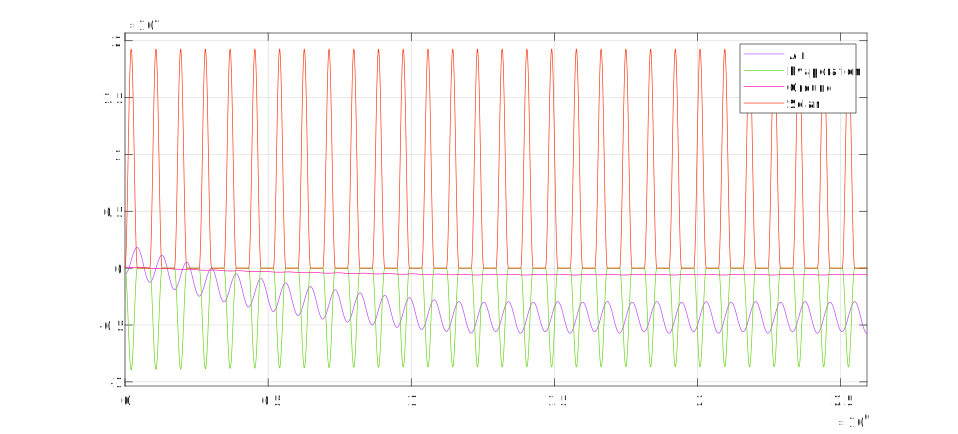
\includegraphics[width=\linewidth]{umgebung-hitze}
	\caption{Durch die Umwelt erzeugte Leistungsverschiebungen}
	\label{fig:umgebung-hitze}
\end{figure}
Auffällig ist, dass die Luft zu Beginn des Prozesses noch Energie zuführt, danach wird aber nur noch entzogen. Dies kommt von der tiefen Starttemperatur des Poolwassers von 10 °C. Nach drei Tagen wird nur noch Energie abgeführt, wodurch schlussfolgern lässt, dass die Wassertemperatur höher ist, als die Lufttemperatur. 

Durch Mitteln der einzelnen Kurven kann bestimmt werden, welche durchschnittliche Leistung bei den einzelnen Einflüsse verloren geht:
\begin{table}[h]
	\begin{tabular}{ll}
		Luft              & - 4340 W                                 \\
		Verdunsten        & - 2232 W                                 \\
		Boden und Wände   & - 0575 W                                 \\
		Sonne             & + 4817 W         						 \\ \hline
		Total			  & - 2330 W
	\end{tabular}                                                           
\end{table}


